\documentclass[varwidth=false, border=2pt]{standalone}

\usepackage{pgfplots}
\usepackage{tikz}

\begin{document}
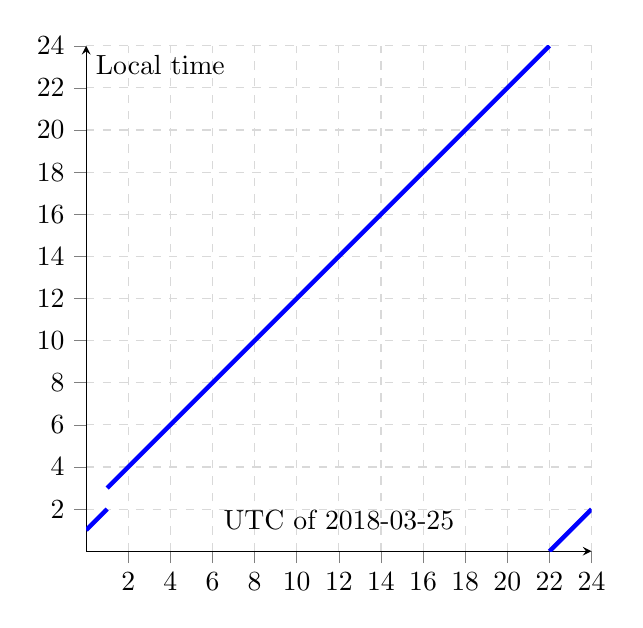
\begin{tikzpicture}
    \begin{axis}[
        axis x line=middle,
        axis y line=middle,
        grid = major,
        width=8cm,
        height=8cm,
        grid style={dashed, gray!30},
        xmin= 0,     % start the diagram at this x-coordinate
        xmax=24,    % end   the diagram at this x-coordinate
        ymin= 0,     % start the diagram at this y-coordinate
        ymax= 24,   % end   the diagram at this y-coordinate
        xlabel=UTC of 2018-03-25,
        ylabel=Local time,
		/pgfplots/xtick={0, 2, ..., 24}, % make steps of length 2
		/pgfplots/ytick={0, 2, ..., 24}, % make steps of length 2
        x label style={at={(axis description cs:0.5,0.1)},anchor=north},
        tick align=outside,
        enlargelimits=false]
      % plot the function
	  \addplot[domain=0:1, blue, ultra thick,samples=20] {x+1};
      \addplot[domain=1:22, blue, ultra thick,samples=20] {x+2};
      \addplot[domain=22:24, blue, ultra thick,samples=20] {x-22};
    \end{axis}
\end{tikzpicture}
\end{document}
